\documentclass[titlepage]{jarticle}
\usepackage[dvipdfmx]{graphicx}
\usepackage{listings}
\usepackage{here}
\usepackage{amsmath}

%
\lstset{
  basicstyle={\ttfamily},
  identifierstyle={\small},
  % commentstyle={\smallitshape},
  keywordstyle={\small\bfseries},
  ndkeywordstyle={\small},
  stringstyle={\small\ttfamily},
  frame={tb},
  breaklines=true,
  columns=[l]{fullflexible},
  numbers=left,
  xrightmargin=0zw,
  xleftmargin=3zw,
  numberstyle={\scriptsize},
  stepnumber=1,
  numbersep=1zw,
  lineskip=-0.5ex,
  language=c
}
\renewcommand{\lstlistingname}{ソースコード}
\makeatletter
\newcommand{\figcaption}[1]{\def\@captype{figure}\caption{#1}}
\newcommand{\tblcaption}[1]{\def\@captype{table}\caption{#1}}
\makeatother
\begin{document}
\section{テーマ}
制御ゼミナールのレポートについて直線を検出するアルゴリズムについて調べC++で実装した.
\section{直線検出のアルゴリズム}
直線検出のアルゴリズムには大きく分けて次の2つあると考えられる.
\begin{enumerate}
  \item Hough変換
  \item LSD(Line Segment Detector)
\end{enumerate}
\subsection{Hough変換}
Hough変換は各点を通る直線が無限個あり,それが様々な方向を向く.
それらの直線の中で画像中の点を最も多く通るものを決定する.
直線の式は,
\begin{equation}
  y = ax + b\\
  r = x \cdot cos(\theta) + y \cdot sin(\theta)\label{equ:r}\\
\end{equation}
の2つがある.この時,$a,b$は任意の定数.$x,y$を座標,
$r$を座標$(x,y)$を通る直線との距離,
$\theta$を座標$(x,y)$を通る直線と垂直に交わり$r$を通る直線とx軸の成す角とする.
また,それぞれの式は図\ref{xy},\ref{rtheta}のように表される.
\begin{figure}[H]
  \begin{minipage}{0.495\hsize}
    \centering
    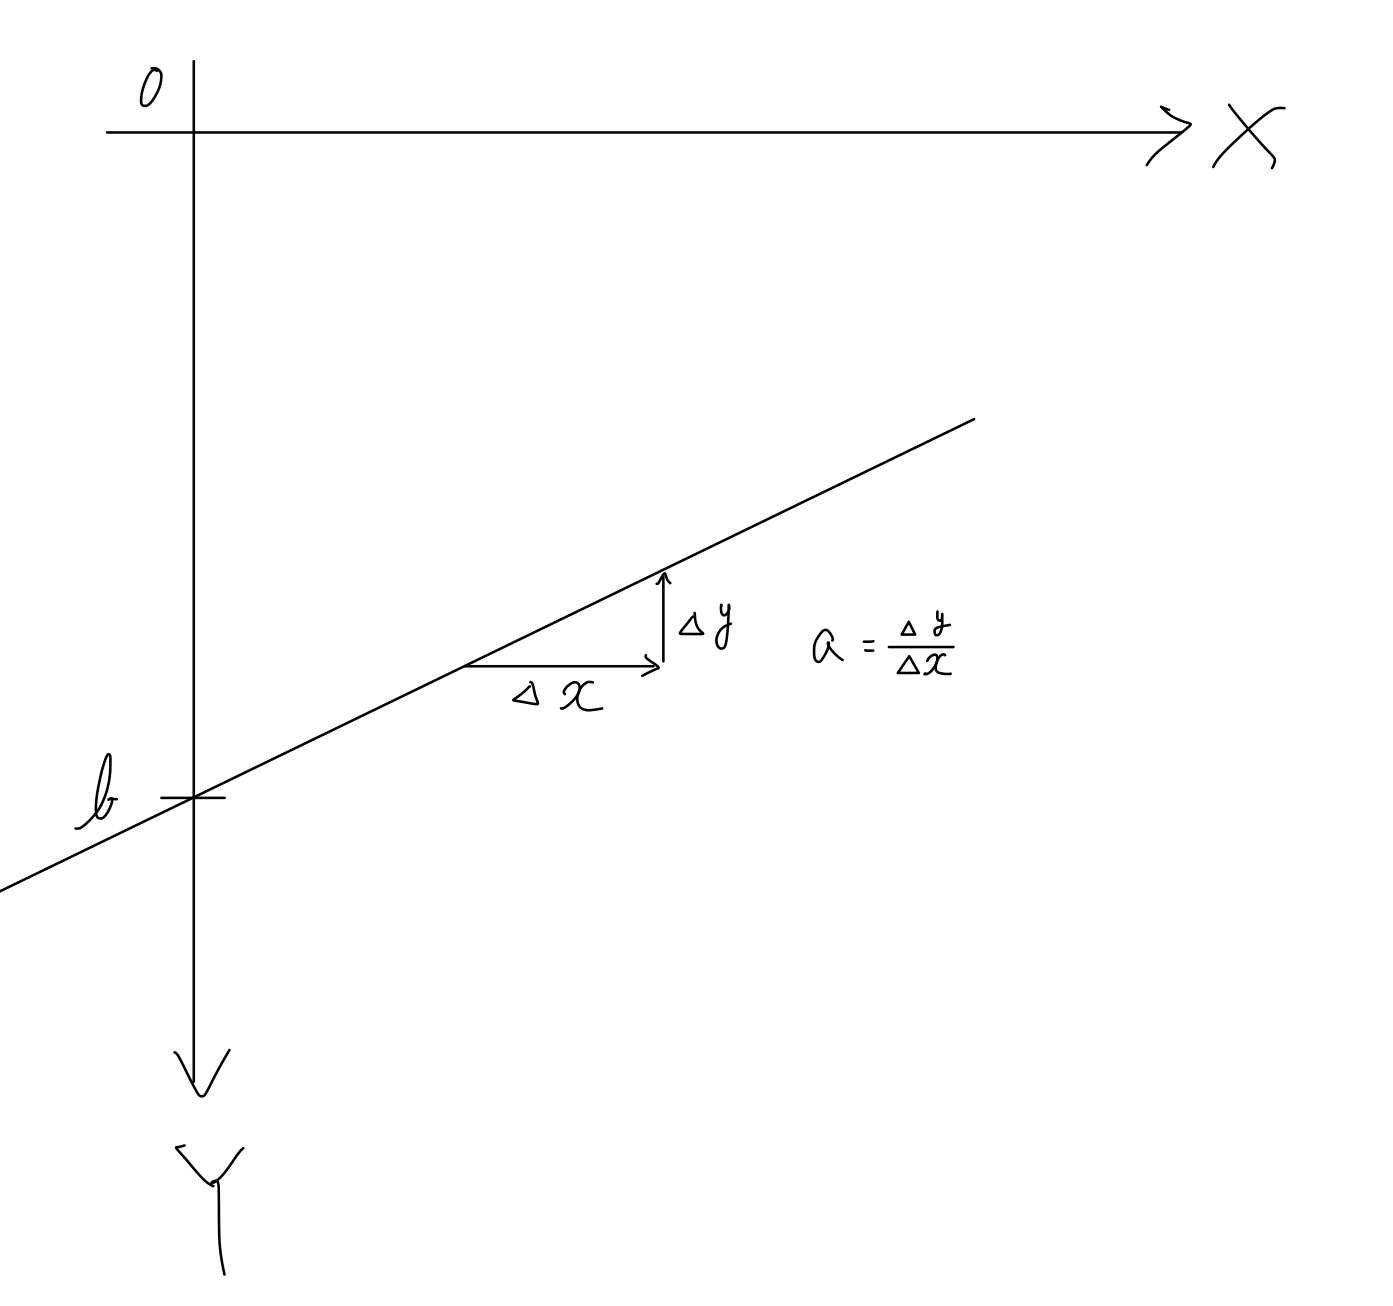
\includegraphics[width=5.5cm]{img/image.png}
    \caption{$y = ax + b$の図}
    \label{xy}
  \end{minipage}
  \begin{minipage}{0.495\hsize}
    \centering
    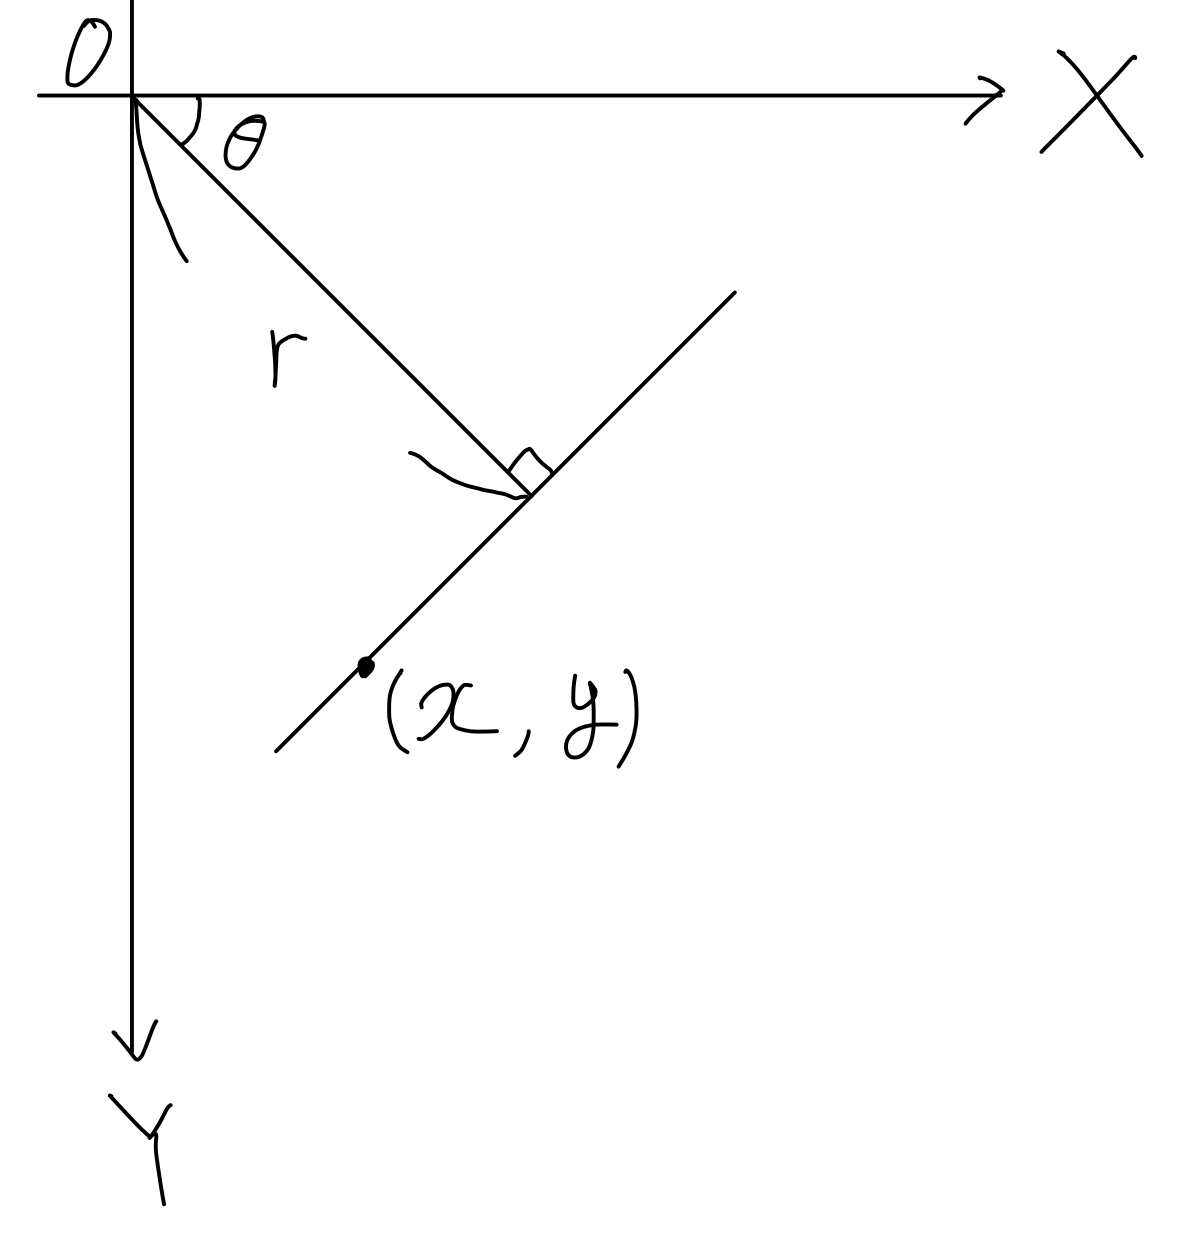
\includegraphics[width=5.5cm]{img/rtheta.png}
    \caption{$r = x \cdot cos(\theta) + y \cdot sin(\theta)$の図}
    \label{rtheta}
  \end{minipage}
\end{figure}
Hough変換では式\eqref{equ:r}を用いて画像内の点を通る直線を$r$と$\theta$で表す.
最も多く使用された$r$と$\theta$のペアによって作られる直線が直線であると考えられる.

\subsection{LSD(Line Segment Detector)}
LSDは画像上の局所的な直線の輪郭を検出することを目的としている.
輪郭とは明暗の変化が十分に早く変化している場所を指している.

\section{実装}
今回はHough変換を実装した.
入力はすでに2値化されたASCII PBMファイルを使用し,
出力は最も多く使用された$r$と$\theta$のペアとする.

\subsection{ソースコード}
ヘッダファイルをソースコード\ref{header}に,
Hough変換の主要部をソースコード\ref{Hough}に示す.
\begin{lstlisting}[caption=header,label=header]
#include <fstream>
#include <iostream>
#include <cmath>
#include <sstream>
#include <string>

using namespace std;

#define SITA 180
\end{lstlisting}
\begin{lstlisting}[caption=Hough Transration,label=Hough]
  int row = ceil(sqrt(xmax * xmax + ymax * ymax));
  int k = 0, distance = 0, rmax, sitamax;
  int** rsita;

  rsita = new int*[row];
  for (i = 0; i < row; i++) {
    rsita[i] = new int[SITA];
    // cout << i << endl;
  }

  for (j = 0; j < row; j++) {
    for (i = 0; i < SITA; i++) {
      rsita[j][i] = 0;
    }
  }

  for (j = 0; j < ymax; j++) {
    for (i = 0; i < xmax; i++) {
      if (matrix[j][i] == 1) {
        for (k = 0; k < SITA; k++) {
          distance = round(i * cos(k * M_PI / 180) + j * sin(k * M_PI / 180));
          if (distance < 0) {
            distance *= -1;
          }
          rsita[distance][k] += 1;
        }
      }
    }
  }

  int max_rsita = 0;

  for (j = 0; j < row; j++) {
    for (i = 0; i < SITA; i++) {
      cout << rsita[j][i] << " ";
      if (max_rsita < rsita[j][i]) {
        max_rsita = rsita[j][i];
      }
    }
    cout << endl;
  }

  for (j = 0; j < row; j++) {
    for (i = 0; i < SITA; i++) {
      if (max_rsita == rsita[j][i]) {
        cout << "r = " << j << ", θ = " << i << "°" << endl;
      }
    }
  }
\end{lstlisting}
このとき,ymaxとxmaxはそれぞれ画像の縦と横の最大の値である.

\subsection{評価方法}
このソースコードを評価するために図\ref{sam1}から\ref{sam4}を用意した.
\begin{figure}[H]
  \begin{minipage}{0.495\hsize}
    \centering
    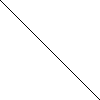
\includegraphics[width=5.5cm]{img/sam1.png}
    \caption{$y = x$の直線のある図}
    \label{sam1}
  \end{minipage}
  \begin{minipage}{0.495\hsize}
    \centering
    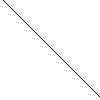
\includegraphics[width=5.5cm]{img/sam2.png}
    \caption{$y = x - 3$の直線のある図}
    \label{sam2}
  \end{minipage}

  \begin{minipage}{0.495\hsize}
    \centering
    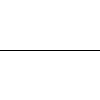
\includegraphics[width=5.5cm]{img/sam3.png}
    \caption{$y = 50$の直線のある図}
    \label{sam3}
  \end{minipage}
  \begin{minipage}{0.495\hsize}
    \centering
    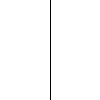
\includegraphics[width=5.5cm]{img/sam4.png}
    \caption{$x = 50$の直線のある図}
    \label{sam4}
  \end{minipage}
\end{figure}
画像はすべて100$\times$100の大きさである.
これらの画像を自作のHough変換のソースコードに入力し,正しい値が出ているか評価する.

\subsection{結果}
図\ref{sam1}から\ref{sam4}の結果を表\ref{tab}に示す.

\begin{table}[H]
  \caption{画像から検出した直線のパラメータ}
  \label{tab}
  \centering
  \begin{tabular}{r|rr}\hline
                & r  & $\theta$° \\\hline\hline
    図\ref{sam1} & 0  & 135       \\
    図\ref{sam2} & 2  & 135       \\
    図\ref{sam3} & 50 & 90        \\
    図\ref{sam4} & 50 & 0         \\\hline
  \end{tabular}
\end{table}

このように出てきている値が概ね問題ないため,ソースコード\ref{Hough}は正しいものであると言える.

\section{考察・感想}
\subsection{考察}
今回作成したHough変換では,$O(N^{3})$になるため計算量が大変多くなる.
また,最も多くの点を含んでいる直線のみしか検出していないため,
画像に一本長い線が入ってしまうとそれしか表示されなくなってしまう.
そのため完璧なものとは言い難い.

これらの改善点として次のようなものが挙げられる.
\begin{enumerate}
  \item 確率モデルを用いて計算する点の量を減らす.
  \item 上位数\%までの直線は表示する.
\end{enumerate}

またこれ以外にも,もう一つの直線検出方法であるLSDを用いてみると良いのではないかと考える.

\subsection{感想}
直線を検出するアルゴリズムについて調査し,C++で実装を行った.
結果としてC++に対する理解と直線検出のアルゴリズムが深まったので良かった.
ただ,当初考えていた直線検出のアルゴリズムとやや違う形になってしまったので,
力不足で実装する時間を十分に作れなかったことを反省したい.

\section*{参考文献}
\begin{enumerate}
  \item 2022資格情報処理研究室ゼミ資料
  \item ハフ変換とLSDによる直線検出の比較\\
        (https://data-analysis-stats.jp/python/ハフ変換とlsdによる直線検出の比較/)
  \item C++の基礎:数学関数の使い方を学ぶ\\
        (https://docwiki.embarcadero.com/Support/ja/C++の基礎:数学関数の使い方を学ぶ)
\end{enumerate}
\end{document}